\documentclass[a4paper,12pt]{article}  % or "report" for larger documents

\usepackage{polski}  % Polish language support
\usepackage[utf8]{inputenc}  % UTF-8 encoding
\usepackage{amsmath, amssymb}  % Math support
\usepackage{float}
\usepackage{graphicx}  % Insert images
\usepackage{hyperref}  % Clickable links
\usepackage{biblatex}  % Bibliography management
\addbibresource{references.bib}  % Reference file
\renewcommand{\figurename}{rys.}

\title{Metody numeryczne, projekt 2:\\ Układy równań liniowych}
\author{Franciszek Fabiński - s197797}
\date{\today}

\begin{document}

\maketitle  % Generates title page

\section{Wstep teoretyczny}

Tematyką drugiego projektu jest rozwiązywanie układów równań liniowych
z wykorzystaniem dwóch metod iteracyjnych (metoda Jacobiego i metoda Gaussa-Seidela) oraz
jednej metody bezpośredniej (faktoryzacji LU). Analiza danych metod będzie
przeprowadzana na danych wywnioskowanych zgodnie ze schematem instrukcji
projektu. 
\smallbreak
W rzeczywistych problemach takie układy równań często nie będą rozmiaru tutaj
analizowanych, lecz znacznie większego, rzędu milionów niewiadomych. W takich
przypadkach najmniejsza optymalizacja algorytmu może przenieść się na
oszczędzenie wielu godzin, dni czy nawet tygodni obliczeń.
\smallbreak
Do zrealizowania projektu wykorzystany został język programowania Python oraz
biblioteka NumPy oraz biblioteka matplotlib do wizualizacji wyników. Wszelkie
operacje na macierzach i wektorach są realizowane z wykorzystaniem
wbudowanych funkcji NumPy, co zapewnia dużą wydajność obliczeń i pozwala skupić
się na implementacji algorytmu.

\pagebreak
\section{Formalizm matematyczny i dane testowe}
Instrukcja projektu używa stałych zależnych od numeru indeksu autora. W
moim przypadku mają one następujące wartości:

\begin{itemize}
  \item $c = 9$
  \item $d = 7$
  \item $e = 7$
  \item $f = 7$
\end{itemize}

Macierz $A$ jest macierzą trójdiagonalną, a wektor $b$ jest wektorem
jednostkowym. Macierz $A$ jest generowana w oparciu o następujący wzór:
\begin{equation}
    A_{i,j} = \begin{cases}
        5+e = 12 & \text{jeśli } i = j \\
        -1 & \text{jeśli } |i - j| < 3 \\
        0 & \text{w przeciwnym razie}
    \end{cases}
\end{equation}

Elementy wektora $b$ są opisane wzorem:
\begin{equation}
    b_i = \sin(i * (f+1)) = \sin(i * 8)
\end{equation}


Macierz $A$ ma rozmiar 1297x1297, a wektor $b$ ma rozmiar 1297x1.
Rozmiar macierzy i wektora jest wyznaczany na podstawie wzoru:
\begin{equation}
    n = 1200 + 10 * c + d = 1200 + 90 + 7 = 1297
\end{equation}

Macierz $A$ ma wymiary $1297 \times 1297$, a wektor $b$ ma wymiary $1297 \times 1$.
\smallbreak

Ostatecznie dane wejściowe wyglądają następująco:

\begin{equation}
  A = \begin{bmatrix}
    12 & -1 & -1 & 0 & 0 & \cdots & 0 & 0 \\
    -1 & 12 & -1 & -1 & 0 & \cdots & 0 & 0 \\
    -1 & -1 & 12 & -1 & -1 &  \cdots & 0 & 0 \\
    0 & -1 & -1 & 12 & -1 & \cdots & 0 & 0 \\
    0 & 0 & -1 & -1 & 12 & \cdots & 0 & 0 \\
    \vdots & \vdots & \vdots & \vdots & \vdots & \ddots & \vdots & \vdots \\
    0 & 0 & 0 & 0 & 0 & \cdots & 12 & -1 \\
    0 & 0 & 0 & 0 & 0 & \cdots & -1 & 12 \\
  \end{bmatrix}
\end{equation}

\begin{equation}
  b = \begin{bmatrix}
    \sin(1 * 8) \\
    \sin(2 * 8) \\
    \sin(3 * 8) \\
    \sin(4 * 8) \\
    \sin(5 * 8) \\
    \vdots \\
    \sin(1297 * 8) \\
  \end{bmatrix}
\end{equation}


\subsection{Metoda bezpośrednia}
Do metody bezpośredniej użyta została faktoryzacja LU.
Faktoryzacja LU polega na rozkładzie macierzy $A$ na iloczyn dwóch
macierzy: $L$ i $U$, gdzie $L$ jest macierzą dolnotrójkątną, a $U$ jest
macierzą górnotrójkątną.
\begin{equation}
    A = LU
\end{equation}

W celu rozwiązania układu równań $Ax = b$ należy wykonać następujące kroki:
\begin{enumerate}
    \item Rozwiązać układ równań $Ly = b$ w celu wyznaczenia wektora $y$.
    \item Rozwiązać układ równań $Ux = y$ w celu wyznaczenia wektora $x$.
\end{enumerate}
Do rozkładu macierzy $A$ na iloczyn macierzy $L$ i $U$ użyta została
metoda Doolittle'a. Rezultatem metody Doolittle'a jest macierz $L$ i $U$,
gdzie diagonalna część macierzy $L$ jest równa 1. Metoda ta jest kosztowna
obliczeniowo, ponieważ wymaga $O(n^3)$ operacji arytmetycznych.
\subsection{Metody iteracyjne}
Do obydwu metod iteracyjnych macierz $A$ powinna być macierzą
przekątniowo dominującą.
Macierz $A$ jest przekątniowo dominująca, jeśli dla każdego wiersza
$A_{ii}$ zachodzi:
\begin{equation}
    |A_{ii}| > \sum_{j \neq i} |A_{ij}|
\end{equation}

\subsubsection{Metoda Jacobiego}
Metoda Jacobiego jest jedną z najprostszych metod iteracyjnych. Polega na
wyznaczeniu wektora $x$ w oparciu o poprzedni wektor $x^{(k)}$.
\begin{equation}
    x^{(k+1)}_i = \frac{1}{A_{ii}} \left( b_i - \sum_{j \neq i} A_{ij} x^{(k)}_j \right)
\end{equation}
Wektor $x^{(k+1)}$ jest wyznaczany na podstawie wektora $x^{(k)}$.

\subsubsection{Metoda Gaussa-Seidela}
Metoda Gaussa-Seidela polega na wyznaczeniu wektora $x$ w oparciu o
poprzedni wektor $x^{(k)}$ oraz aktualny wektor $x^{(k+1)}$.
\begin{equation}
  x^{(k+1)}_i = \frac{1}{A_{ii}} \left( b_i - \sum_{j = 1}^{i-1} A_{ij}
  x^{(k+1)}_j - \sum_{j = i+1}^{n} A_{ij} x^{(k)}_j \right)
\end{equation}

\section{Analiza wyników}

\subsection{Poprawnie uwarunkowana macierz}

Poniższe wyniki przedstawione są dla macierzy wygenerowanej zgodnie z wzorem
(1), wg. którego macierz okazuje się być przekątniowo dominująca.


\begin{figure}[H]
  \centering
  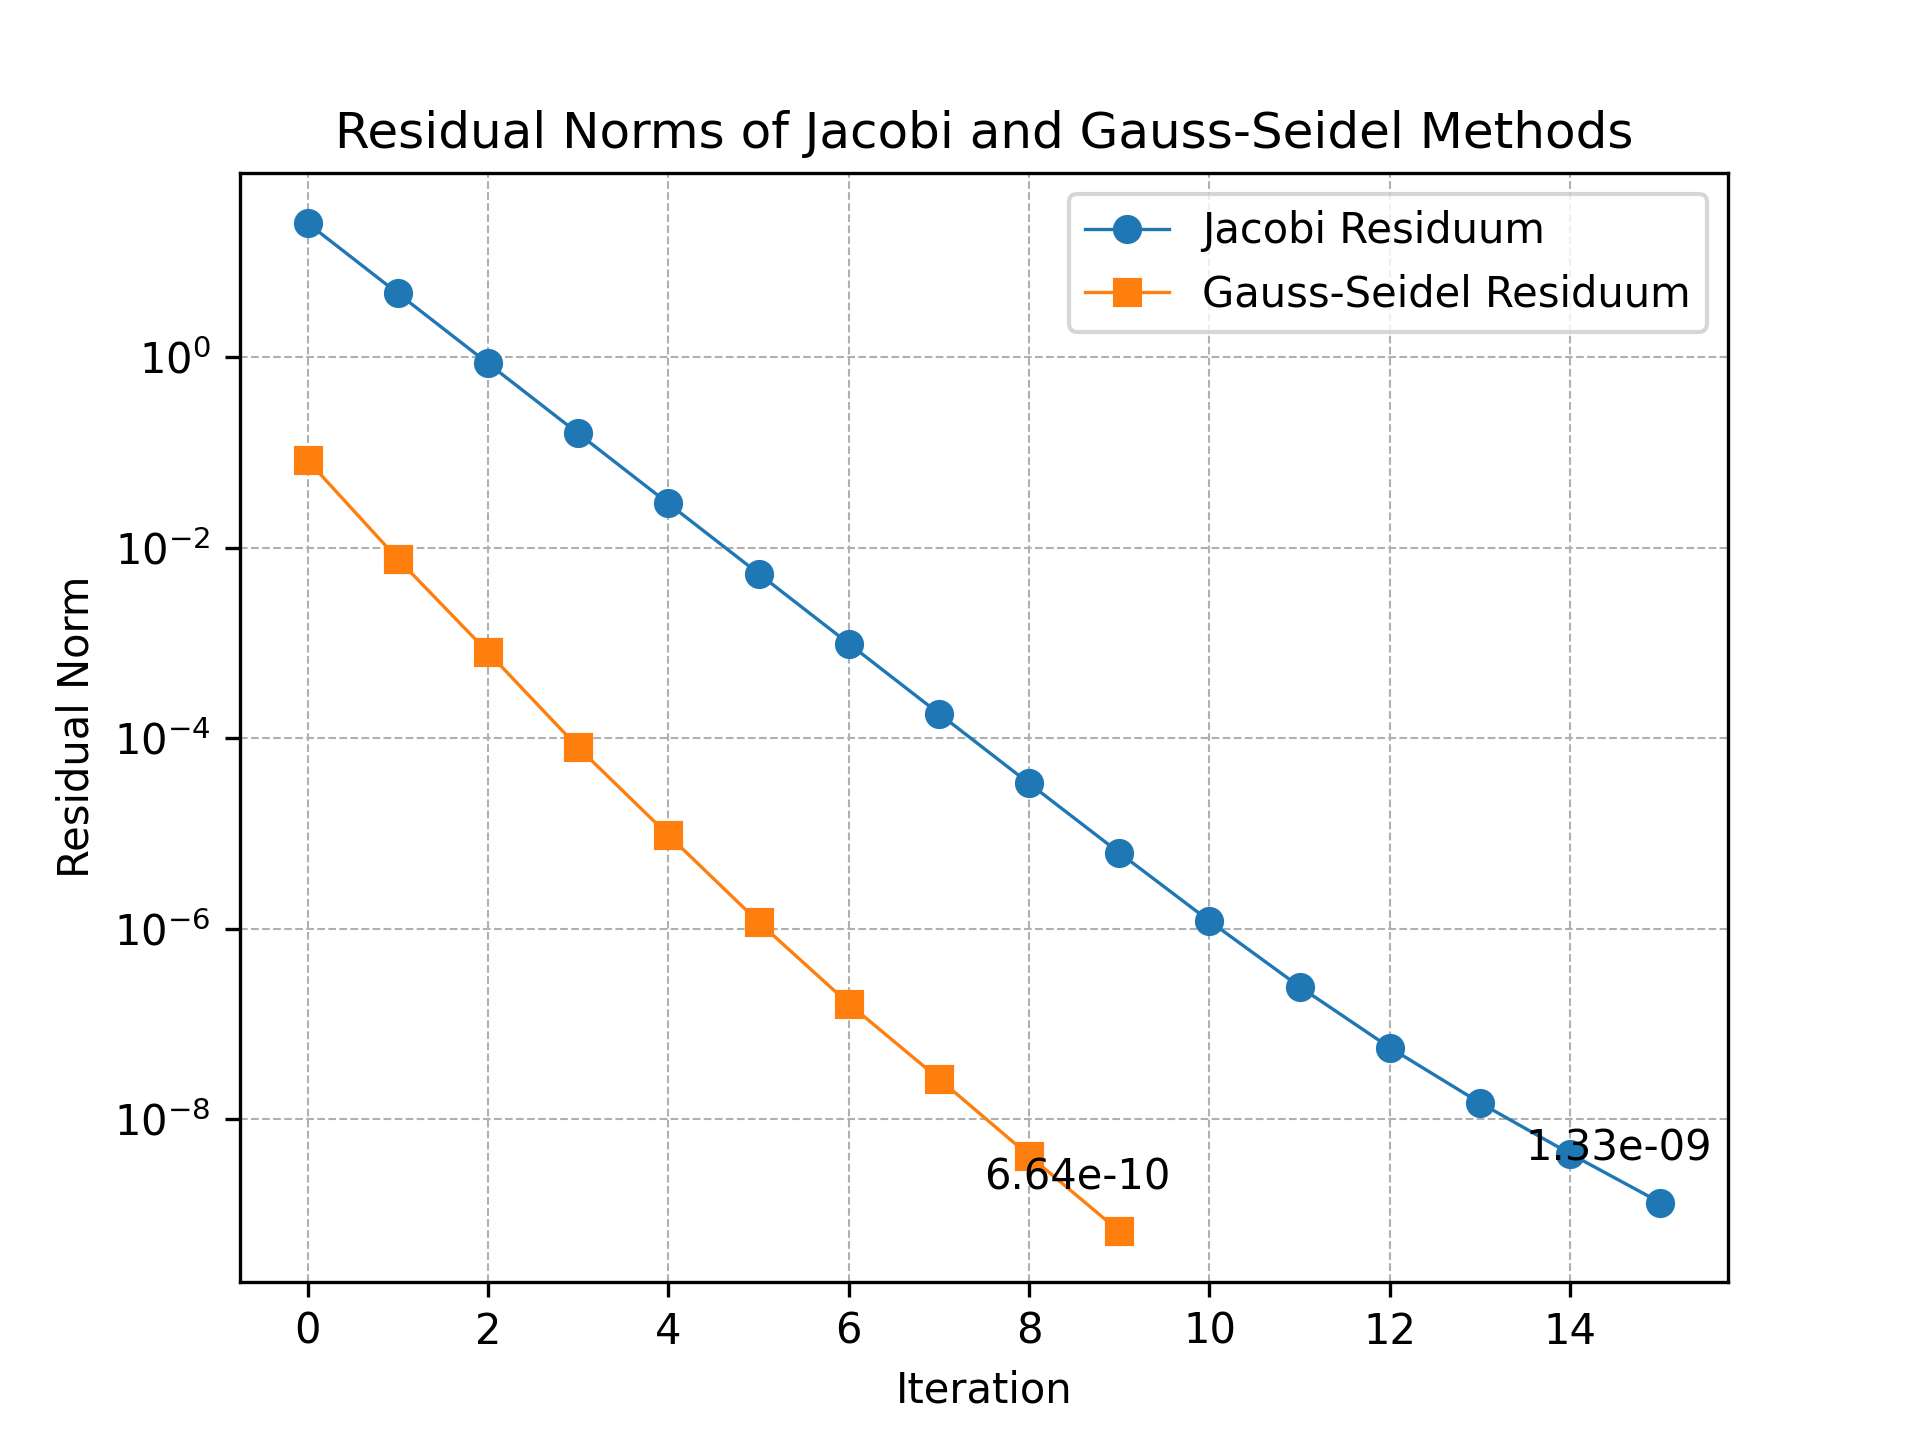
\includegraphics[width=0.8\textwidth]{./graphs/residuals_task_a.png}
  \caption{Wykres reszt dla metody Jacobiego i Gaussa-Seidela}
\end{figure}
Krzywe z rys. 1 przedstawiają zbieżność obu metod iteracyjnych. Metoda 
Gaussa-Seidela zbiega szybciej niż metoda Jacobiego, przez co potrzebowała
ona jedynie 10 iteracji do osiągnięcia wyniku w granicach tolerancji
($10^{-9}$), o 5 iteracji mniej niż metodzie Jacobiego. W tym przypadku metodzie 
Gaussa-Seidela obliczenie wyniku zajęło \textbf{0.06} sekundy, a metodzie
Jacobiego \textbf{0.09}.

\subsection{Źle uwarunkowana macierz}
W przypadku źle uwarunkowanej macierzy, która nie jest przekątniowo
dominująca, zastosowanie metod iteracyjnych skutkuje brakiem
ich zbieżności.

\begin{figure}[H]
  \centering
  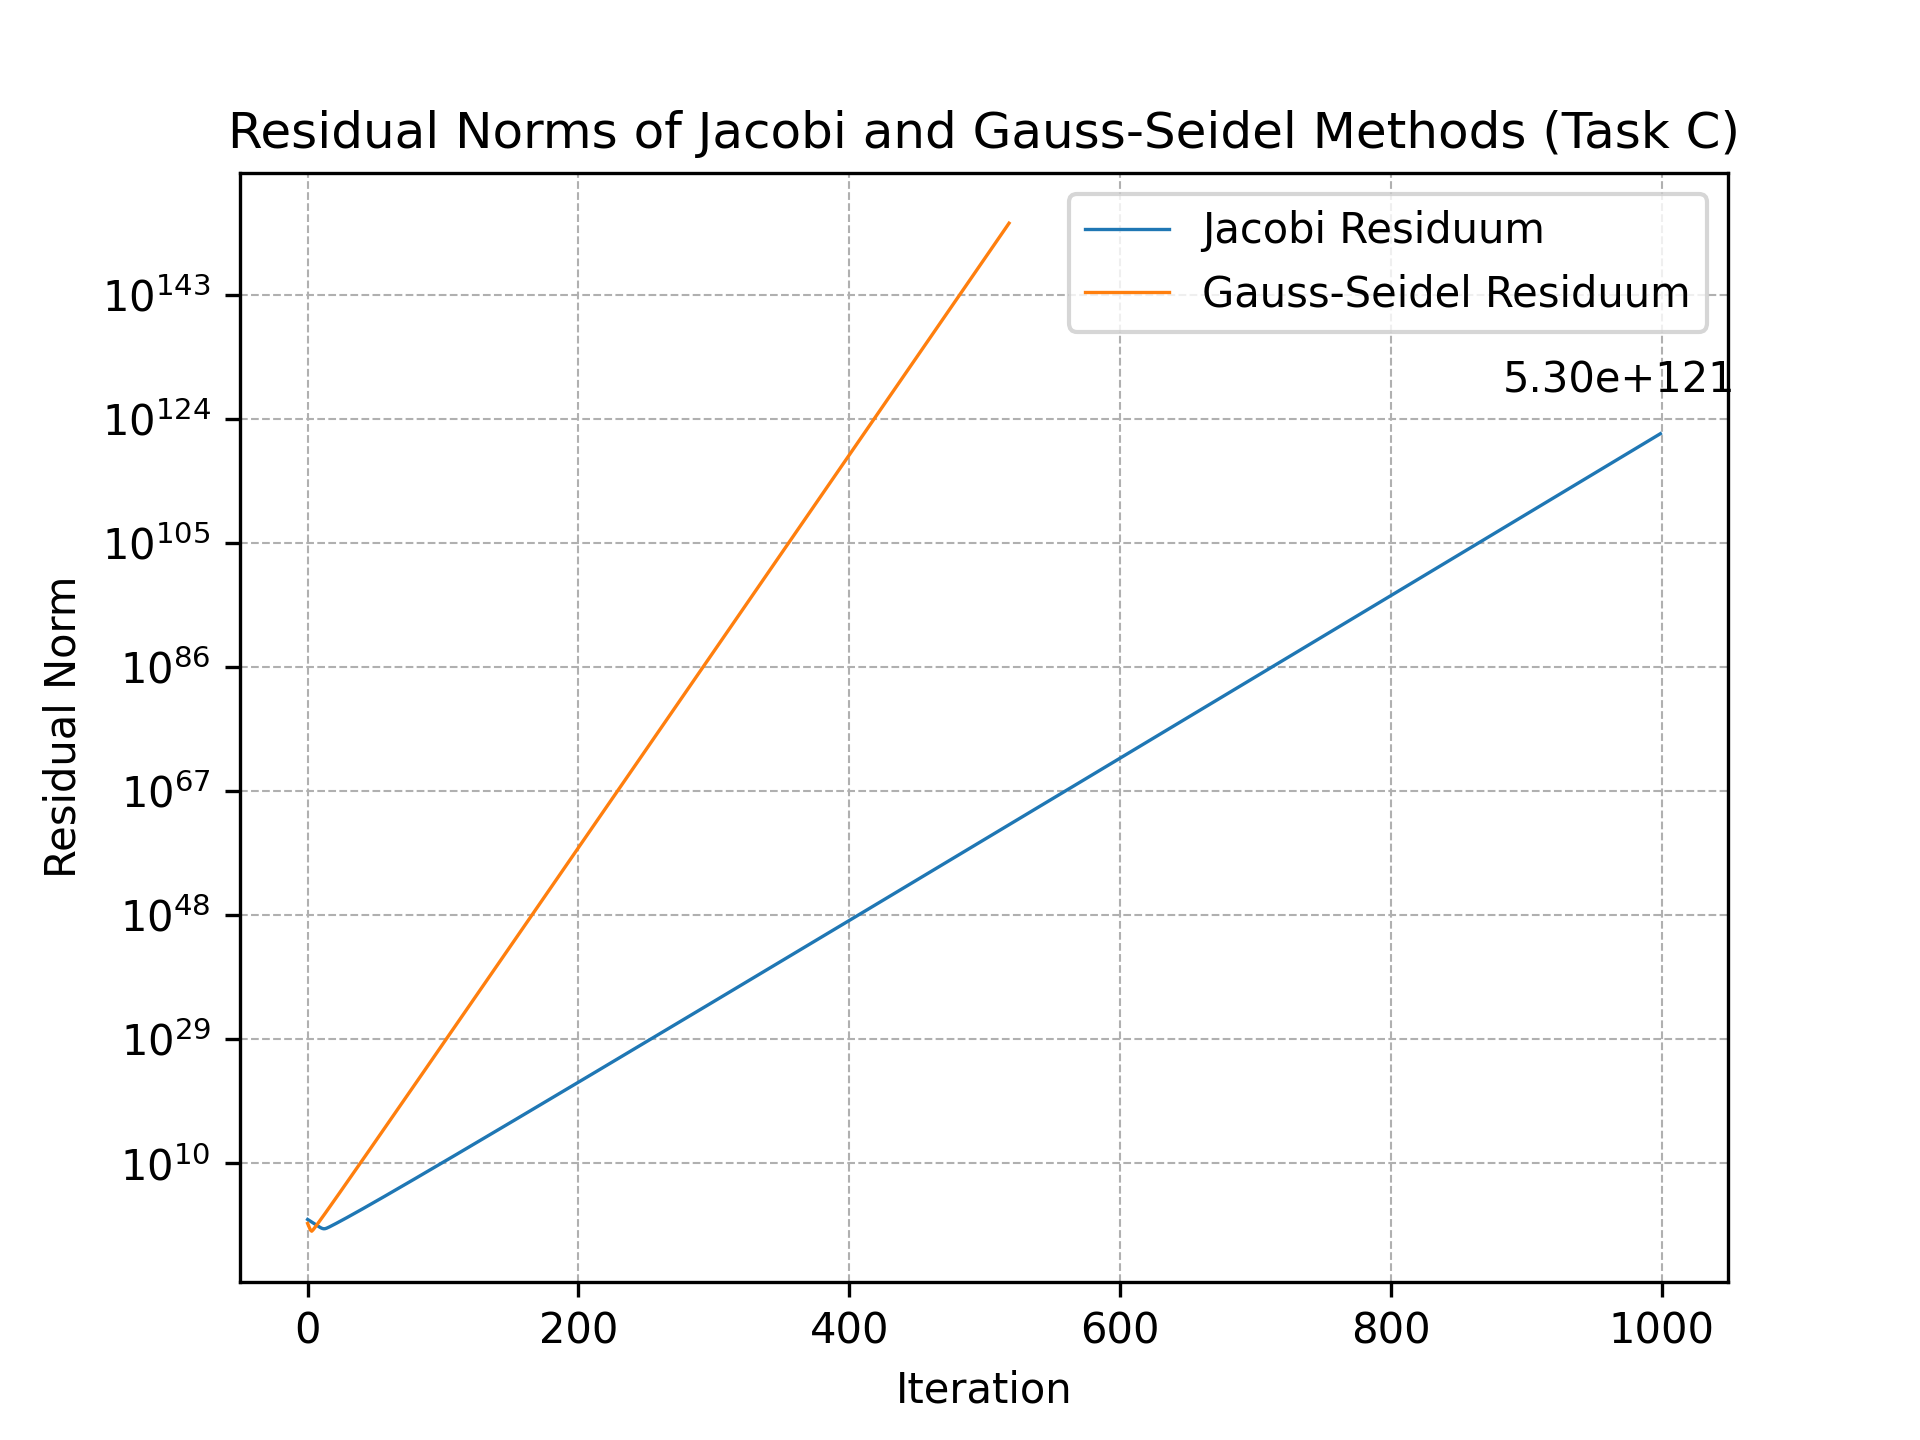
\includegraphics[width=0.8\textwidth]{./graphs/residuals_task_c.png}
  \caption{Wykres reszt dla metody Jacobiego i Gaussa-Seidela dla źle
  uwarunkowanej macierzy}
\end{figure}

Na rys. 2 przedstawione są krzywe zbieżności dla źle uwarunkowanej
macierzy. Jak widać, metoda Gaussa-Seidela rośnie szybciej niż metoda
Jacobiego, lecz obydwie rosną wykładniczo. Dalsze iteracje powstrzymał
odgórny limit iteracji, który został ustawiony na 1000.

\subsection{Faktoryzacja LU}
W przypadku rozwiązywania układu zawierającego źle uwarunkowaną macierz
niemożliwe jest zastosowanie metod iteracyjnych. W takim przypadku
zastosować można jedynie metodę bezpośrednią, która w tym przypadku
zajęła \textbf{195.13} sekundy. Norma residuum wyniosła \textbf{$1.68*10^{-10}$}.

\pagebreak
\section{Porównanie czasów obliczeń}
Przedstawione wyniki są czasami obliczeń dla macierzy dobrze
uwarunkowanych. Dodatkowo dla pewności poprawnych wyników, dla każdej
metody zwiekszono liczbę iteracji do 1000000.

\begin{figure}[H]
  \centering
  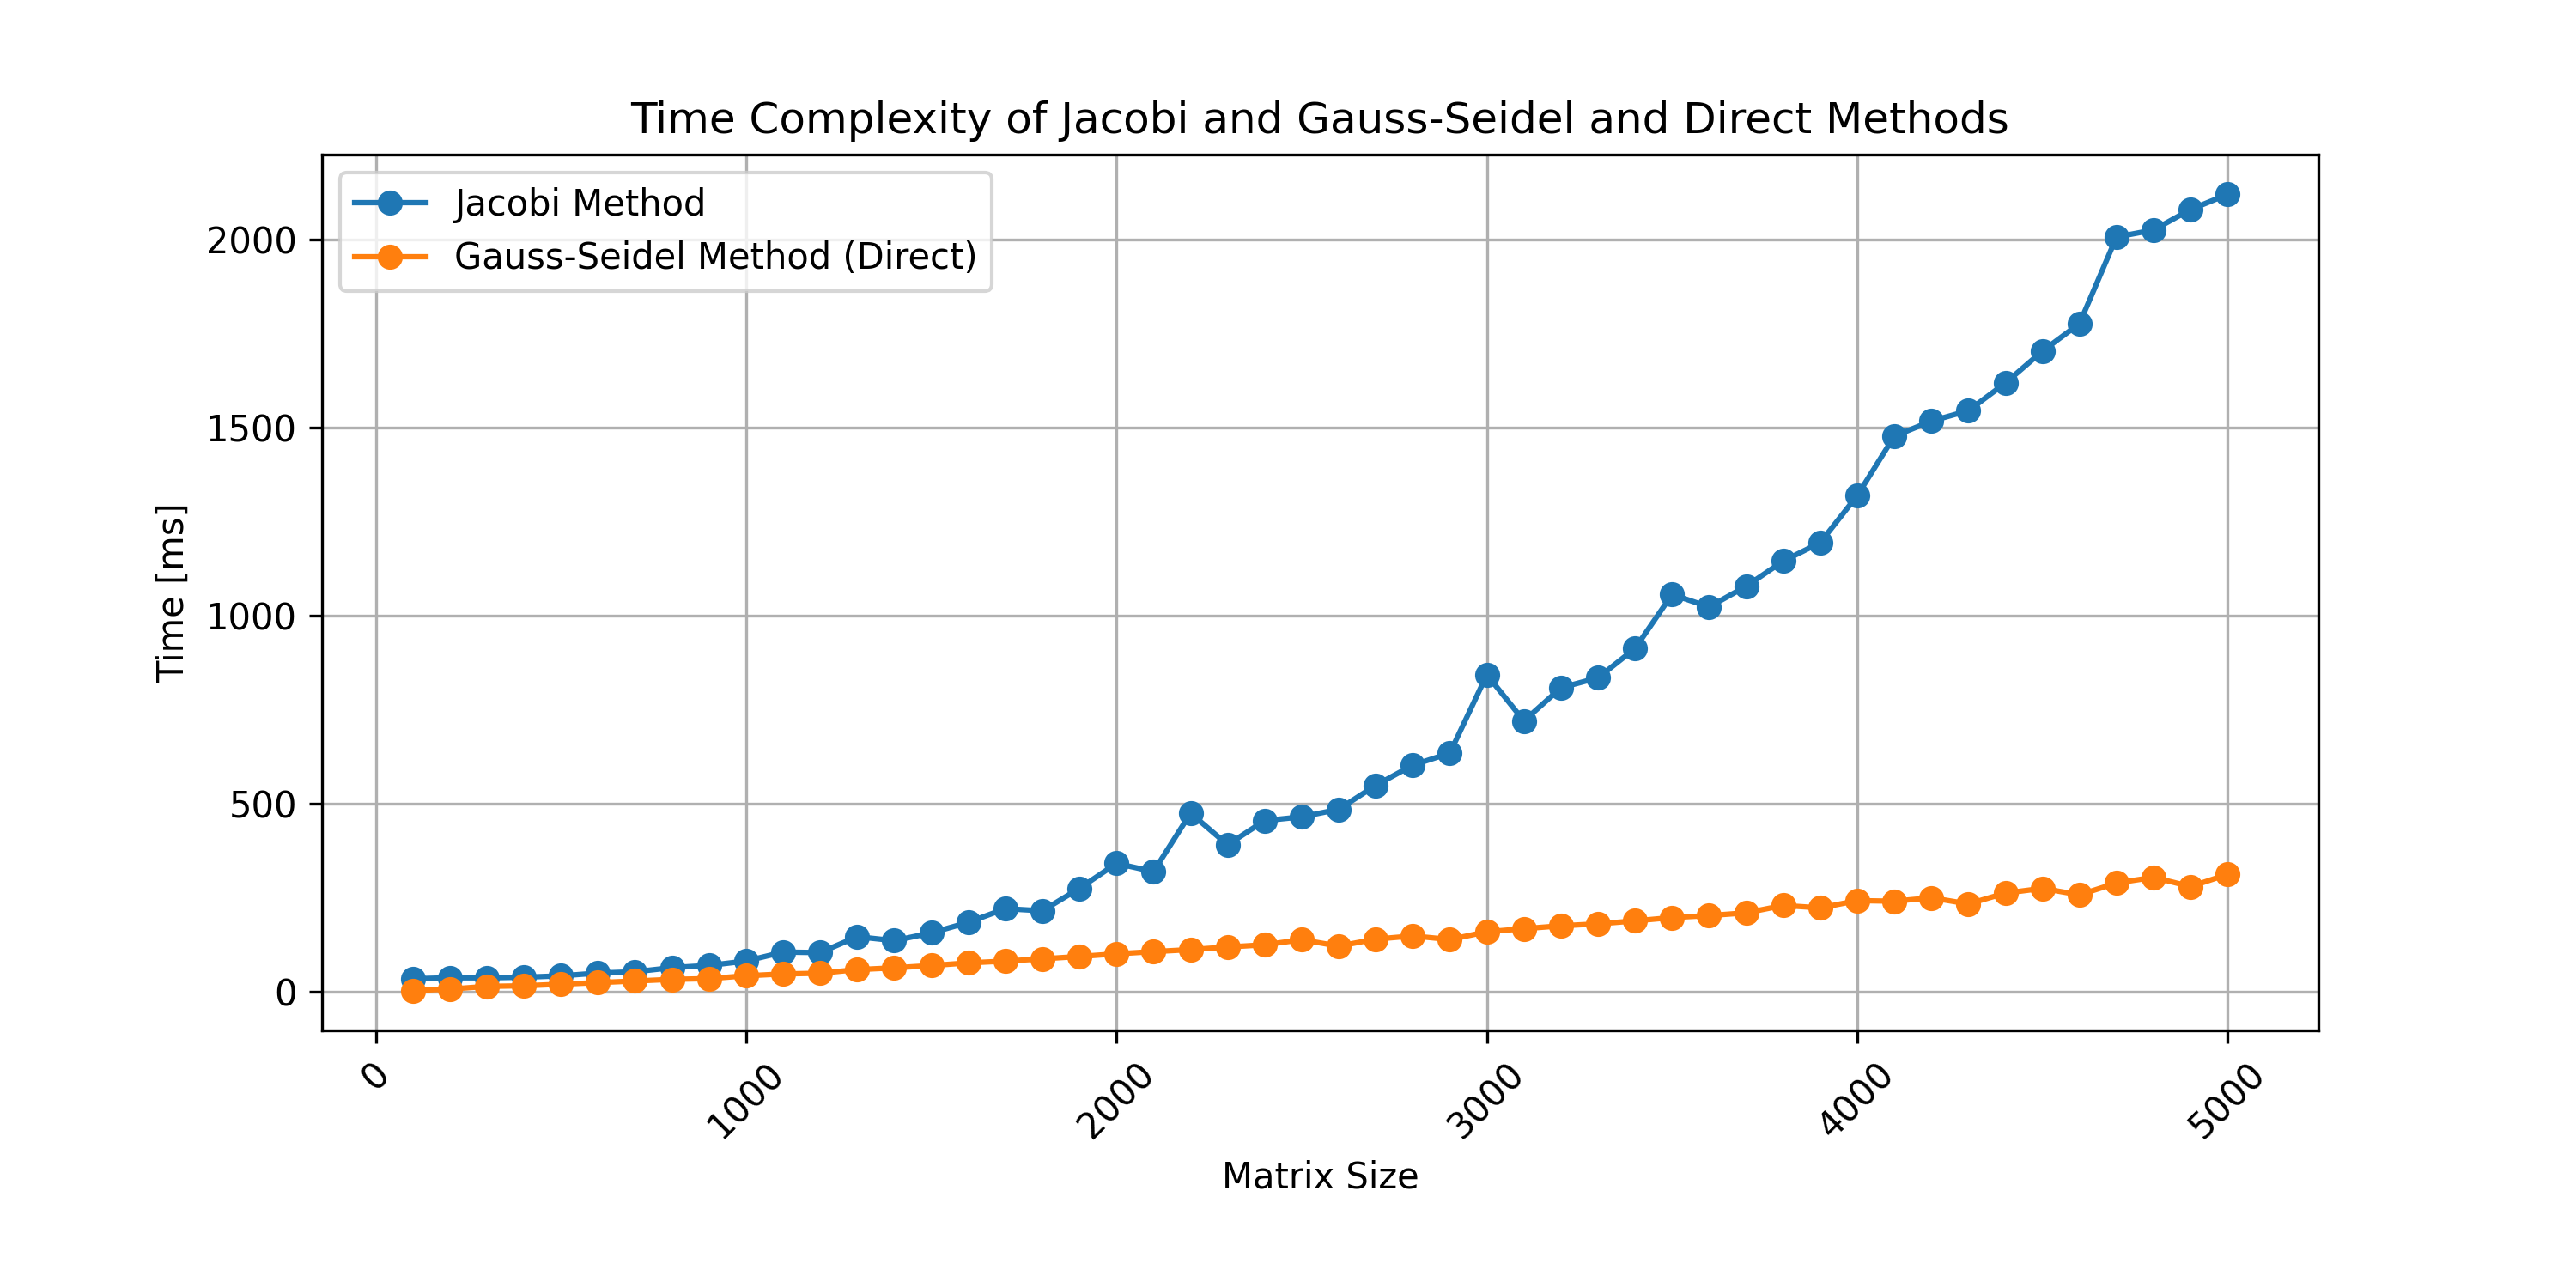
\includegraphics[width=0.8\textwidth]{./graphs/time_complexity_linear.png}
  \caption{Czasy obliczeń w skali liniowej}
\end{figure}

Na rys. 3 przedstawione są czasy obliczeń dla każdej z metod 
w skali liniowej. Jak widać, metoda Jacobiego jest znacznie wolniejsza
od metody Gaussa-Seidela.

\begin{figure}[H]
  \centering
  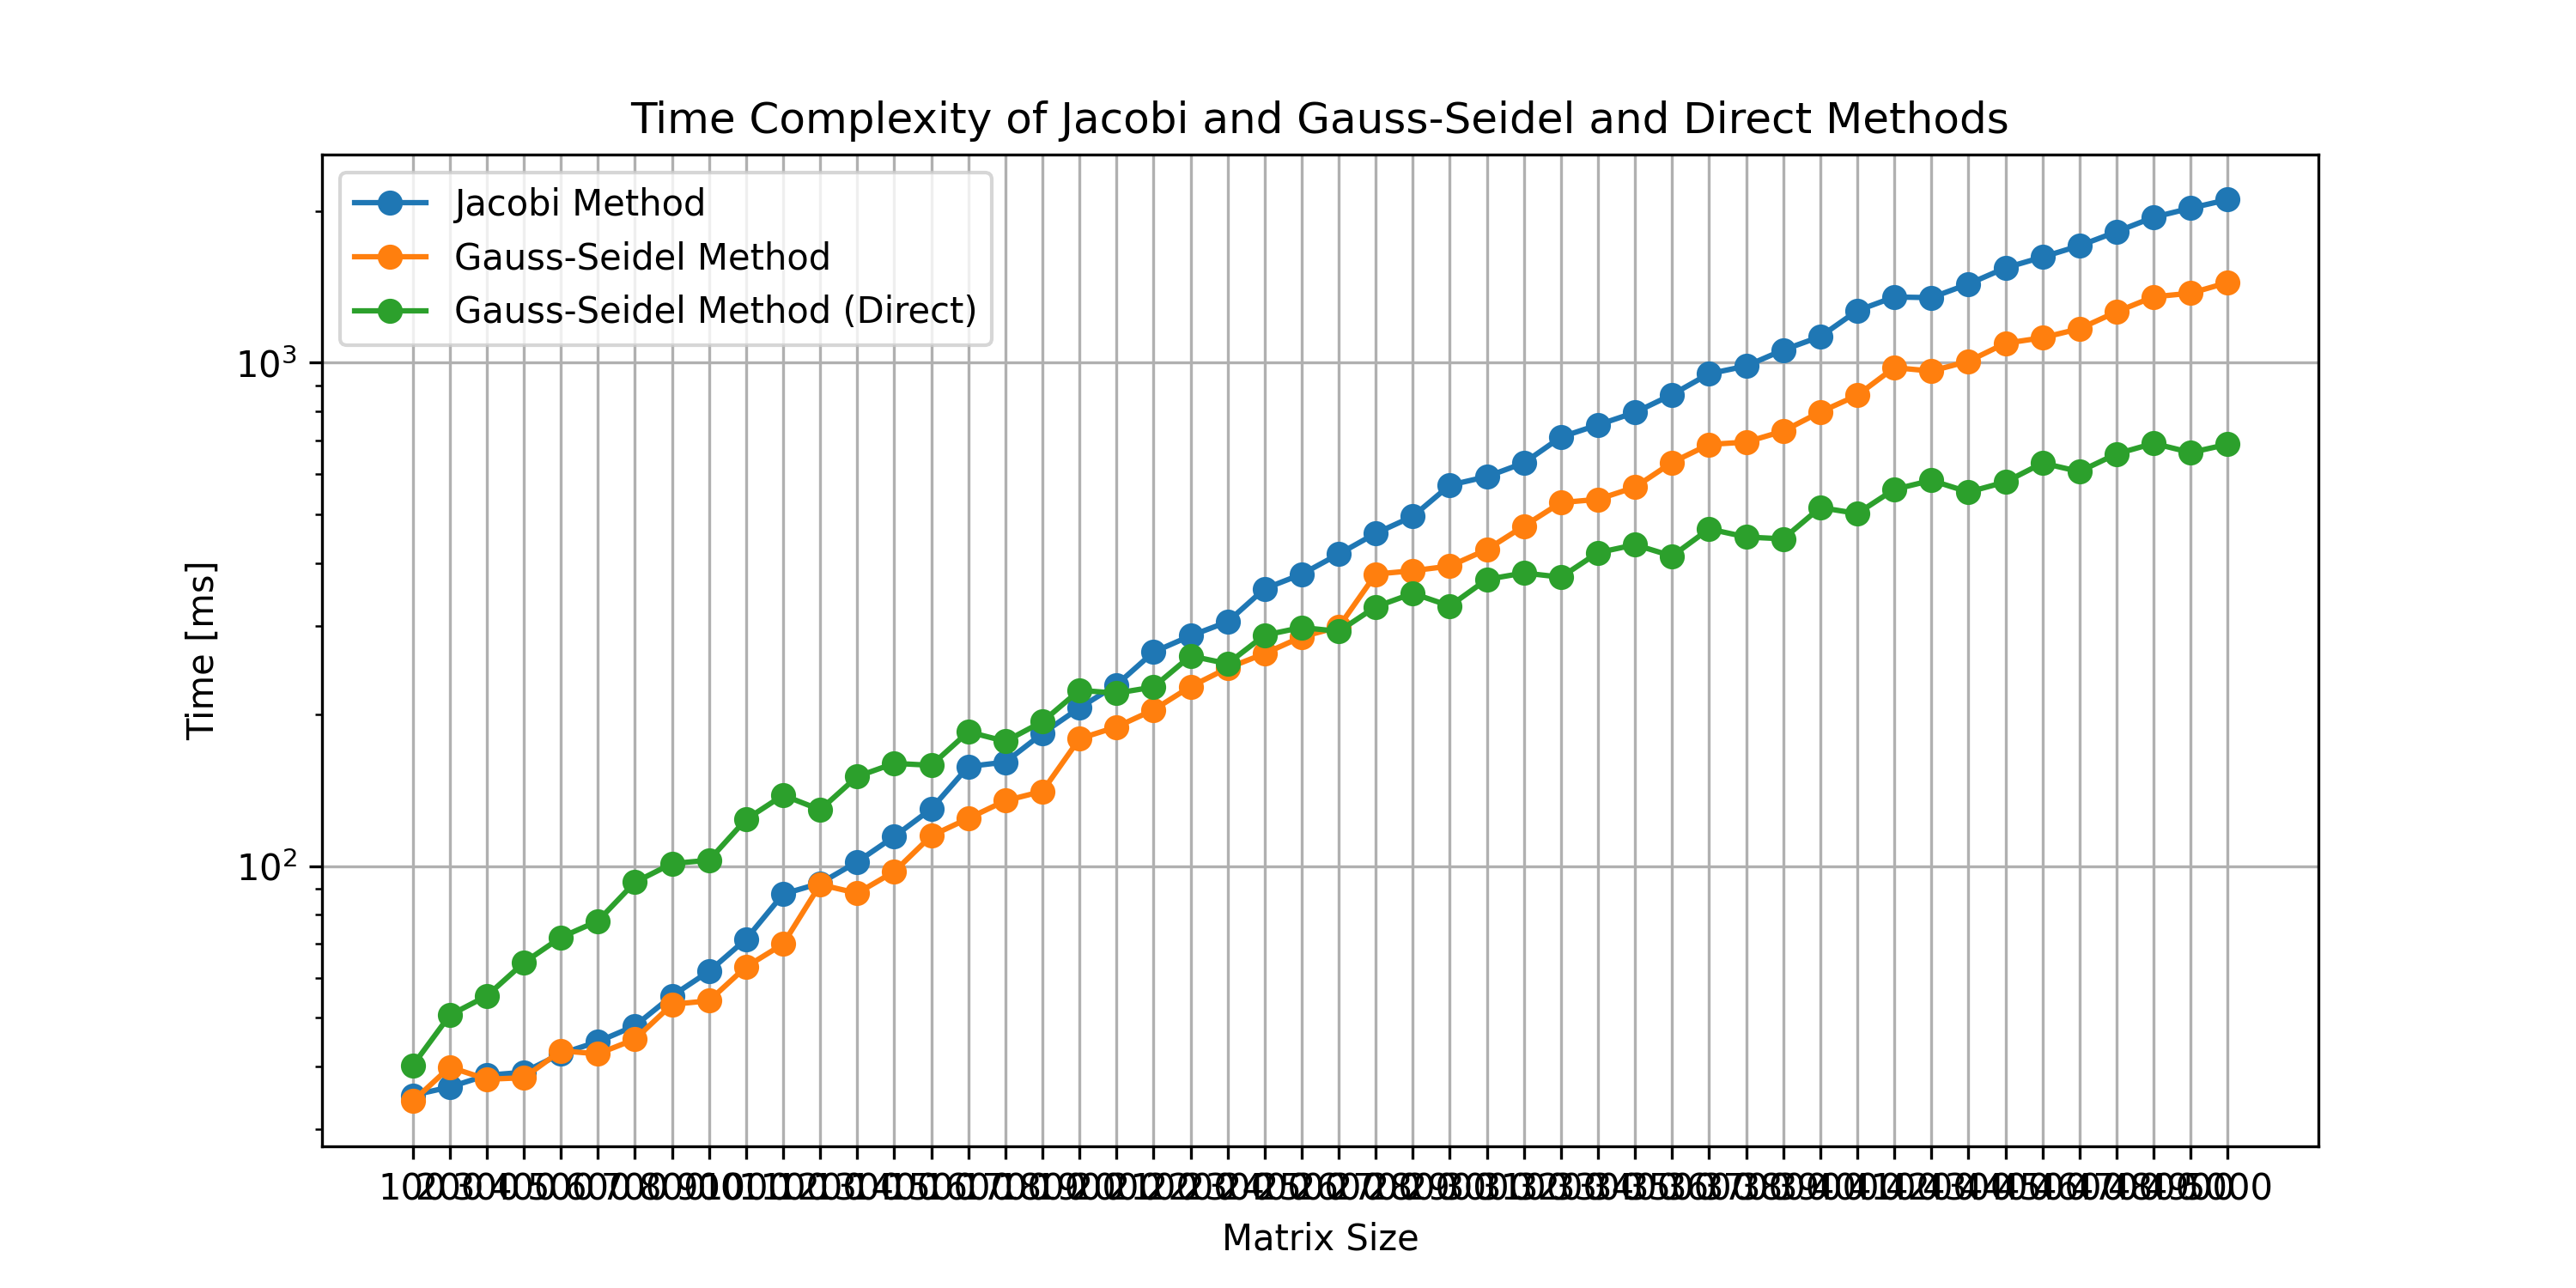
\includegraphics[width=0.8\textwidth]{./graphs/time_complexity.png}
  \caption{Czasy obliczeń w skali logarytmicznej}
\end{figure}

\pagebreak

\section{Podsumowanie}
W projekcie przedstawione zostały trzy metody rozwiązywania układów równań
liniowych. Metoda Jacobiego i metoda Gaussa-Seidela są metodami
iteracyjnymi, które są stosunkowo proste w implementacji, lecz wymagają
przekątniowo dominującej macierzy. W przypadku źle uwarunkowanej
macierzy, która nie jest przekątniowo dominująca, metody te nie 
zbiegają. Użycie metody bezpośredniej jest znacznie wolniejsze, lecz
czasami niezbędne. 

\begin{thebibliography}{9}
\bibitem{LU decomposition}
Geeks for Geeks (2023) \emph{LU Decomposition}, \url{https://www.geeksforgeeks.org/doolittle-algorithm-lu-decomposition/}.
\bibitem{Iterative methods}
Yousef Saad \emph{Iterative Methods for Sparse Linear Systems}.
\end{thebibliography}

\printbibliography

\end{document}
